\documentclass[spanish]{textolivre}

% metadata
\journalname{Texto Livre}
\thevolume{17}
%\thenumber{1} % old template
\theyear{2024}
\receiveddate{\DTMdisplaydate{2024}{3}{26}{-1}}
\accepteddate{\DTMdisplaydate{2024}{9}{10}{-1}}
\publisheddate{\today}
\corrauthor{Raquel Barragán Sánchez}
\articledoi{10.1590/1983-3652.2024.51787}
%\articleid{NNNN} % if the article ID is not the last 5 numbers of its DOI, provide it using \articleid{} commmand 
% list of available sesscions in the journal: articles, dossier, reports, essays, reviews, interviews, editorial
\articlesessionname{articles}
\runningauthor{Barragán Sánchez y Murta}
%\editorname{Leonardo Araújo} % old template
\sectioneditorname{Daniervelin Pereira}
\layouteditorname{João Mesquita}

\title{La seguridad en Internet como parte de la competencia digital ciudadana: revisión sistemática}
\othertitle{Segurança na Internet como parte da competência digital do cidadão: revisão sistemática}
\othertitle{Internet security as part of citizen digital competence: systematic review}

\author[1]{Raquel Barragán Sánchez ~\orcid{0000-0001-6336-2728}\thanks{Email: \href{mailto:rbarragan@us.es}{rbarragan@us.es}}}
\author[2]{Luís Manuel da Cruz Murta ~\orcid{0000-0002-4395-2664}\thanks{Email: \href{mailto:lmurta@ipbeja.pt }{lmurta@ipbeja.pt }}}
\affil[1]{Universidad de Sevilla, facultad de ciencias de la Educación, departamento de Didáctica y Organización Educativa, Sevilla, España.}
\affil[2]{Centro de Investigação em Qualidade de Vida (CIEQV), Instituto Politécnico de Beja, Beja, Portugal.}

\addbibresource{article.bib}
\usepackage{array}

\begin{document}
\maketitle
\begin{polyabstract}
\begin{abstract}
La formación en competencia digital es considerada un eje prioritario en España y en Europa en los últimos años. Dentro de esta, se incluye la seguridad en Internet como se refleja en el área 4 del marco de competencia digital europeo Digcomp. El objetivo de esta investigación es analizar el estado de la cuestión con el fin de detectar posibles lagunas que se están produciendo en la investigación de esta temática y así poder impulsar futuras líneas de investigación en las que hay que profundizar. Se ha seguido la metodología de investigación bibliográfica según los parámetros definidos en la declaración PRISMA. Las bases de datos utilizadas para la búsqueda han sido Web of Science, Scopus y ERIC. Tras un proceso de búsqueda, cribado y selección de la información se ha obtenido una muestra de 30 artículos científicos publicados entre 2013 y 2023. Se han realizado análisis descriptivos y de contenido para dar respuesta a los interrogantes planteados. Los resultados muestran que la seguridad digital se está trabajando de forma parcial y en ocasiones no se vincula a la competencia digital ciudadana. Se reconocen como principales responsables de su formación a docentes y familias, aunque estos no disponen de herramientas suficientes para facilitar la mediación responsable. El ámbito universitario es un entorno prioritario tanto para la formación de los futuros docentes como para la formación de los futuros profesionales. En conclusión, se reconoce la importancia del contexto educativo para hacer frente a la necesidad formativa en seguridad digital, pero de momento no existen respuestas globales y reconocidas que encuentren reflejo en los marcos competenciales.

\keywords{Competencia digital \sep Seguridad Digital \sep Uso seguro de internet \sep Educación en seguridad \sep TIC}
\end{abstract}

\begin{portuguese}
\begin{abstract}
A formação em competências digitais é considerada uma prioridade em Espanha e na Europa nos últimos anos. Isto inclui a segurança da Internet, tal como refletido na área 4 do quadro europeu de competências digitais Digcomp. O objetivo desta pesquisa é analisar o estado da questão para detectar possíveis lacunas que estão ocorrendo na pesquisa deste tema e assim poder promover futuras linhas de pesquisa nas quais devemos nos aprofundar. A metodologia de pesquisa bibliográfica foi seguida de acordo com os parâmetros definidos na declaração PRISMA. As bases de dados utilizadas para a busca foram Web of Science, Scopus e ERIC. Após processo de busca, triagem e seleção de informações, obteve-se uma amostra de 30 artigos científicos publicados entre 2013 e 2023. Foram realizadas análises descritivas e de conteúdo para responder às questões colocadas. Os resultados mostram que a segurança digital está sendo trabalhada parcialmente e, por vezes, não está vinculada à competência digital do cidadão. Os professores e as famílias são reconhecidos como os principais responsáveis pela sua formação, embora não possuam ferramentas suficientes para facilitar uma mediação responsável. O ambiente universitário é um ambiente prioritário tanto para a formação de futuros professores como para a formação de futuros profissionais. Concluindo, reconhece-se a importância do contexto educativo para responder à necessidade de formação em segurança digital, mas neste momento não existem respostas globais e reconhecidas que se reflitam nos quadros de competências.

\keywords{Competência digital \sep Segurança digital \sep Uso seguro da internet \sep Educação em segurança \sep TIC}
\end{abstract}
\end{portuguese}

\begin{english}
\begin{abstract}
Digital Competence Training is considered a priority in Spain and Europe in recent years. This includes Internet security, as reflected in area 4 of the European Digital Competence Framework, Digcomp. The objective of this research is to analyze the current state of the issue to detect possible gaps in the research on this topic and thus promote future lines of research that need to be deepened. The bibliographic research methodology followed the parameters defined in the PRISMA statement. The databases used for the search were Web of Science, Scopus, and ERIC. After a process of searching, screening, and selecting information, a sample of 30 scientific articles published between 2013 and 2023 was obtained. Descriptive and content analyses were carried out to answer the questions posed. The results show that digital security is being addressed partially and sometimes not linked to citizen digital competence. Teachers and families are recognized as the main responsible for its training, although they do not have sufficient tools to facilitate responsible mediation. The university environment is a priority both for the training of future teachers and for the training of future professionals. In conclusion, the importance of the educational context is recognized to address the training need in digital security, but at the moment there are no global and recognized responses reflected in the competence frameworks.

\keywords{Digital competence \sep Digital security \sep Safe internet use \sep Security education \sep ICT}
\end{abstract}
\end{english}
\end{polyabstract}

\section{Introducción}
La Sociedad de la Información ha transformado radicalmente nuestra vida y la forma en que interactuamos con el mundo. Todos los ámbitos sociales se han visto afectados por los grandes cambios introducidos por las Tecnologías Digitales por lo que el dominio de la competencia digital se ha vuelto un aspecto fundamental para afrontar la vida en la actualidad. Los ciudadanos deben desarrollar competencias que les permitan adaptarse a las necesidades que les plantea el entorno social actual \cite{villarreal2019competencias}.

El uso de las tecnologías digitales ofrece multitud de ventajas que posibilitan una ciudadanía activa pero también conlleva riesgos para los que debe estar preparado, de tal forma que se haga un uso de las Tecnologías de la Información y la Comunicación (TIC) responsable, ético y seguro.

En este contexto, la creación de un marco de la competencia digital que facilite y enmarque las diferentes dimensiones y competencias que son necesarias adquirir es fundamental. Dichos marcos permiten también realizar diagnósticos sobre el desarrollo competencial y enfocar los esfuerzos formativos a aquellas áreas donde se observa más dificultad.

El Marco DigComp, se ha desarrollado por la Comisión Europea y se ha convertido en un referente para muchos países porque define las competencias digitales necesarias para una participación activa, crítica y responsable en la sociedad digital. Se compone de cinco áreas principales: Información y Datos, Comunicación y Colaboración, Creación de Contenido Digital, Seguridad y Resolución de Problemas \cite{cabero2023nativos}. Como se puede observar en la \Cref{fig1}, el marco de la competencia digital no se centra únicamente en el dominio de habilidades técnicas, como la búsqueda de información en línea o el uso de herramientas digitales, sino que también se resaltan habilidades críticas y reflexivas, como la evaluación de la calidad de la información en línea, el uso responsable de datos personales y la identificación de posibles riesgos y amenazas en línea.

\begin{figure}[h!]
\centering
\begin{minipage}{\textwidth}
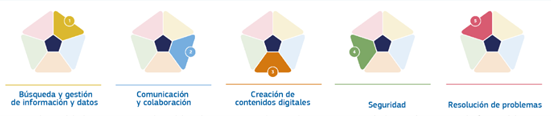
\includegraphics[width=\textwidth]{Fig1.png}
\caption{Áreas y competencias de DigComp.}
\label{fig1}
\source{\textcite{comision2022digcomp}}
\end{minipage}
\end{figure}

Si nos fijamos en el área competencial 4 se reflejan todas aquellas competencias que están vinculadas al área de seguridad con las Tecnologías Digitales (ver \Cref{fig2}). Esto implica que la seguridad en la red conlleva el desarrollo de conocimientos, habilidades y actitudes vinculadas a la protección de los dispositivos, protección de datos personales y privacidad, protección de la salud y el bienestar y la protección medioambiental.

\begin{figure}[h!]
\centering
\begin{minipage}{0.5\textwidth}
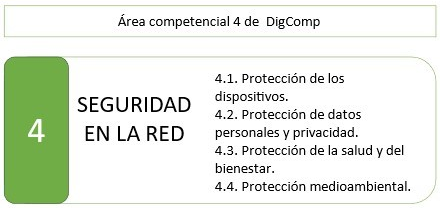
\includegraphics[width=\textwidth]{Fig2.png}
\caption{Áreas y competencias de DigComp.}
\label{fig2}
\source{Área competencia 4 de DigComp.}
\end{minipage}
\end{figure}

En cuanto a la protección de contenidos, es importante tener en cuenta que no todo lo que está en internet puede ser usado sin permiso y que todo lo que subimos es susceptible de ser usado y compartido, por lo que es importante el registro de la propiedad y el reconocimiento de las distintas licencias que podemos encontrar. La protección de dispositivos se ha centrado tradicionalmente en el uso de suit o software de seguridad, que, aunque resultan de gran ayuda, debe hacerse mayor hincapié en la realización estrategias humanas que permiten minimizar los riegos de forma personalizada y en diferentes contextos.

La protección de datos personales y privacidad es otro de los temas clave en cuanto a la seguridad en internet. Es importante concienciar de que toda información que sea altamente sensible nunca debe ser compartida en la Red. Existe normativa sobre la privacidad y opciones que nos permiten regular quién puede acceder a los datos y el uso que se puede hacer de ellos, pero también es cierto que existen muchas infracciones de seguridad y filtraciones ilícitas de datos que, si bien pueden ser denunciadas, los daños a veces son irreparables.

La protección de la salud y el bienestar hace referencia a las amenazas para el bienestar físico y psicológico durante el uso de las tecnologías digitales. Puede incluirse aquí todo lo relacionado a ciberacoso y todo un repertorio de ciberamenazas a las que nos enfrentamos como pueden ser Bullying, Sexting, Grooming... \cite{reset2022problemas} así como a otras enfocadas a la adicción tecnológica o adicciones en general, que ya existían, pero que el uso de internet ha contribuido a una mayor globalización, como las ciberapuestas.

Finalmente, el área de seguridad se centra además en el uso de las tecnologías y la protección medioambiental. Es altamente desconocido el impacto que provoca el uso de las tecnologías en el medio por lo que es necesario concienciar de que es importante hacer un uso responsable de las tecnologías evitando impacto irreparable en el medio ambiente. Los Objetivos de Desarrollo Sostenible hacen alusión a esta temática que cada vez coge más fuerza y está siendo más trabajada \cite{barragan2020teaching,tucho2020impacto,silva2023nivel}.

Cabe destacar que el marco digcomp reconoce diferentes niveles de dominio, por lo que se contempla no únicamente la realización de un uso autónomo de estrategias de seguridad, sino que es necesario alcanzar el nivel en el que el ciudadano es capaz de protegerse y ayudar a otras personas/instituciones a hacerlo. Asimismo, los diferentes niveles contemplan desde el reconocimiento del propio riesgo hasta la proposición creativa de soluciones de protección y adaptación a diferentes contextos.

La integración del Marco DigComp en la educación también implica la formación de los docentes. Esta cuestión supone una doble complejidad. El profesorado debe aprender las competencias vinculadas a la ciudadanía digital, pero, además, también deben aprender a enseñar en competencias a su futuro alumnado. Vinculado a esta necesidad se desarrollan distintos marcos de competencia digital docente en Europa \cite{redecker2017european,intef2017marco}; donde también toman relieve la formación en competencias vinculadas a la seguridad digital. Esto incluye el fomento del respeto a la privacidad y la seguridad en línea, la promoción de la igualdad y la diversidad en línea, y la conciencia sobre el impacto social y medioambiental de la tecnología \cite{rodriguez2023evaluacion}.

Teniendo en cuenta todo lo desarrollado y la importancia que adquiere la seguridad digital dentro de la competencia digital ciudadana y la competencia digital docente, el objetivo que se plantea para este estudio es revisar el estado de la cuestión en este tema para detectar posibles lagunas que se están produciendo en la investigación de esta temática y así poder impulsar futuras líneas de investigación en las que hay que profundizar. Es importante destacar que este estudio trata conocer cómo se está trabajando la seguridad digital dentro de la competencia digital, no se han realizado búsquedas independientes de temas concretos sobre seguridad como pueden ser ciberacoso, adicción, etc.

\section{Preguntas de investigación}\label{sec-normas}
La presente investigación está guiada por las siguientes preguntas o interrogantes:

\begin{enumerate}
    \item ¿Cómo se distribuyen los estudios sobre la seguridad en internet en los 10 últimos años?
    \item ¿Qué áreas de la seguridad digital se están investigando con mayor intensidad?
    \item ¿Qué países están realizando estudios sobre el tema?
    \item ¿En qué contexto se desarrollan las investigaciones?
    \item ¿Cuáles son los principales resultados que han obtenido los estudios analizados?
    \item ¿Qué perspectiva de futuro se presentan en los estudios analizados?
\end{enumerate}

\section{Material y métodos}\label{sec-conduta}
Existen diferentes tipos de revisiones de literatura \cite{grant2009typology}, la metodología seguida en este estudio se enmarca dentro del análisis bibliométrico seguido de un análisis cualitativo de cada artículo resultante para dar respuesta a las preguntas que se plantean en esta investigación \cite{delgado2023revision}. Para la realización del presente trabajo, se decidió optar por el método de investigación indicado por las directrices de la Declaración Preferred Reporting Items for Systematic Reviews and Meta-Analyses (PRISMA). Adoptado por la Asociación Americana de Psicología (APA), este método nos aporta un marco sistemático de acciones a seguir para validar la confiabilidad de los resultados obtenidos \cite{yepez2021declaracion}.   

\subsection{Procedimento y análisis utilizados}
Las búsquedas se han realizado en las bases de datos Web of Science, Scopus y ERIC. Los tópicos que se han utilizado para las búsquedas están en inglés, ya que se considera el idioma más inclusivo según las bases de datos utilizadas. Han sido los siguientes: (Digital Safety) AND (Internet Use) AND (Digital Competence). Todos los artículos analizados cuentan con resumen y palabras clave en inglés, aunque el idioma que utilizan para el texto completo es en su mayoría inglés, también se han analizado algunos escritos en castellano, ruso y turco. Otros presentan la doble vertiente de inglés y su idioma de origen (ver \Cref{tbl1}).

Los criterios de inclusión han sido, artículos científicos, publicados en los 10 últimos años. Debido a que la búsqueda se ha realizado a final del año 2023, hemos incluido También el año 2013. No se han tenido en cuenta el número de citas. También se ha tenido en cuenta el libre acceso en la Base ERIC y, en Wos y Escopus que tenga acceso al menos a resumen.

Atendiendo a los descriptores mencionados se han aplicado los siguientes filtros de búsqueda:

\begin{itemize}
    \item Intervalo de publicación: ajuste temporal: 2013--2023.
    \item Tipo de documentos: artículos científicos.
    \item Idioma del artículo: sin restricción
    \item Idioma del resumen y palabras clave: inglés
    \item Estudios con ítem(s) relacionado(s) con el área competencial de seguridad propuesto en el marco europeo DigComp.
\end{itemize}

El procedimiento de búsqueda y análisis ha constado de varias fases. En primer lugar, se ha realizado una búsqueda independiente en cada base de datos indicada (Web of Science, Scopus y ERIC) se han aplicado los criterios de inclusión, posteriormente se han depurado las duplicidades y finalmente, se ha realizado un análisis de cada artículo atendiendo al título y resumen para comprobar que se ciñe a la temática objeto de estudio. Finalmente, se ha trabajado con una muestra total de 30 artículos que han sido descargados creando una base de datos (Ver \Cref{tbl1}).

\begin{table}[htbp]
\begin{threeparttable}
\centering
\caption{Distribuição dos lemas das 10 predicações mais frequentes, por gênero.}
\label{tbl1}
\begin{tabular}{l >{\raggedright\arraybackslash}p{10cm} l}
\toprule
& Artículos analizados & Idioma \\ 
\midrule
1 & \textcite{isrokatun2022digital} & Inglés \\ 
2 & \textcite{ogegbo2021assessment} & Inglés \\
3 & \textcite{takavarasha2018navigating} & Inglés \\
4 & \textcite{mark2021invitation} & Inglés \\
5 & \textcite{mahadir_digital_2021} & Inglés \\
6 & \textcite{escoda_digital_2021} & Inglés \\
7 & \textcite{jwaifell2018proper} & Inglés \\
8 & \textcite{hazar2018digital} & Inglés \\
9 & \textcite{schlebbe2018selecting} & Inglés \\
10 & \textcite{kaban2020secure} & Inglés \\
11 & \textcite{baeva2020safety} & Inglés \\
12 & \textcite{torres2022indicators} & Inglés \\
13 & \textcite{potyrała2021teachers} & Inglés \\
14 & \textcite{quintana2020transmedia} & Inglés \\
15 & \textcite{soldatova2020digital} & Inglés \\
16 & \textcite{hinojo-lucena_sharenting:_2020} & Inglés y Castellano \\
17 & \textcite{thoma_communication_2019} & Inglés \\
18 & \textcite{chelysheva2017basic} & Inglés \\
19 & \textcite{arrufat2019competence} & Castellano \\
20 & \textcite{torres2019intervencion} & Castellano \\
21 & \textcite{filkina_profiles_2023} & Ruso \\
22 & \textcite{stiakakis_exploring_2022} & Inglés \\
23 & \textcite{tomczyk_parents_2021} & Inglés \\
24 & \textcite{garcia-gutierrez_aproximacion_2013} & Castellano \\
25 & \textcite{alonso-ferreiro_actitudes_2019} & Castellano \\
26 & \textcite{skobeltsina_russian_2021} & Ruso \\
27 & \textcite{tomczyk_parents_2017} & Turco e inglés \\
28 & \textcite{martinez-de-morentin_risks_2021} & Inglés \\
29 & \textcite{soldatova_parental_2019} & Ruso \\
\bottomrule
\end{tabular}
\source{Elaboración propia.}
\end{threeparttable}
\end{table}

A continuación, se ha realizado un análisis cuantitativo de aquellos ítems que lo permiten, realizando una descripción de datos fundamentales, posteriormente se ha realizado un análisis del contenido de cada artículo que conforma la muestra para dar respuesta a las preguntas planteadas. La \Cref{fig3} muestra un resumen del método aplicado.

\begin{figure}[h]
\centering
\begin{minipage}{0.75\textwidth}
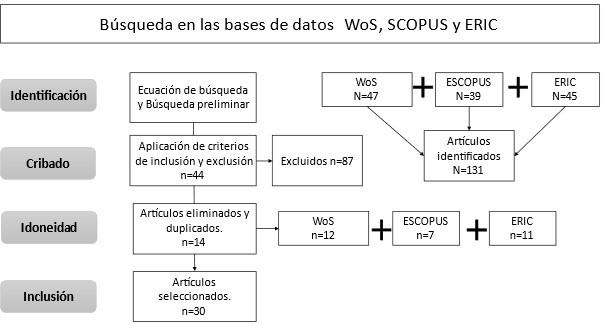
\includegraphics[width=\textwidth]{Fig3.png}
\caption{Proceso de revisión.}
\label{fig3}
\source{basado en \textcite{yepez2021declaracion}.}
\end{minipage}
\end{figure}

\section{Resultados}\label{sec-fmt-manuscrito}
Los resultados se muestran organizados para dar respuesta a las preguntas de investigación u objetivos anteriormente planteados.


\subsection{¿Cómo se distribuyen los estudios sobre la seguridad en internet en los 10 últimos años?}\label{sec-formato}
Como se puede apreciar en la \Cref{fig4}, hay pocos estudios que se interesen por el uso seguro de internet antes de 2017, es a partir de este año que la temática empieza a cobrar importancia culminando en el año 2021 donde se observa un notable crecimiento. Esto puede ser debido a dos aspectos que se consideran claves en esta temática, el desarrollo del marco europeo de la competencia digital (publicada su primera versión en 2017) y el confinamiento e incidencia de la pandemia del coronavirus.

\begin{figure}[h]
\centering
\begin{minipage}{0.65\textwidth}
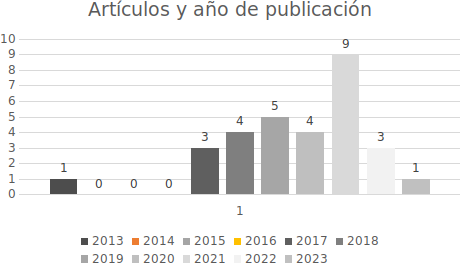
\includegraphics[width=\textwidth]{Fig4.png}
\caption{Año de publicación.}
\label{fig4}
\source{Elaboración propia.}
\end{minipage}
\end{figure}

\subsection{¿Qué áreas de la seguridad digital se están investigando con mayor intensidad?}\label{sec-modelo}
Para realizar el análisis del área referida a la seguridad digital, hemos utilizado las 4 categorías basadas en el marco competencia digital europeo DIGCOMP y se ha añadido una quinta categoría que ha sido necesaria a raíz del análisis de los artículos que componen la muestra. Se definen a continuación:

\begin{itemize}
    \item Categoría 1: Protección de dispositivos y contenidos digitales
    \item Categoría 2: Protección de datos personales y privacidad
    \item Categoría 3: Protección de la Salud y el bienestar
    \item Categoría 4: Protección medioambiental
    \item Categoría 5: Protección en internet sin profundizar en aspectos concretos. Aunque se reconoce la importancia de la seguridad dentro de la alfabetización digital, no se concretan aspectos más allá de las normas de conductas o prevención de delitos digitales sin especificar.
\end{itemize}

Los resultados se muestran en la \Cref{fig5}.

\begin{figure}[h!]
\centering
\begin{minipage}{0.65\textwidth}
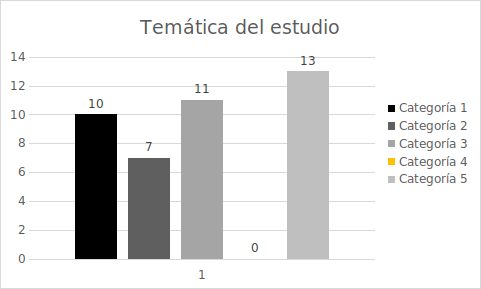
\includegraphics[width=\textwidth]{Fig5.png}
\caption{Temática de los estudios.}
\label{fig5}
\source{Elaboración propia.}
\end{minipage}
\end{figure}

En lo que respecta a la temática concreta de estudio, encontramos que muchos de los estudios abordan la seguridad digital desde una perspectiva genérica. Por otra parte, la categoría 3 y la categoría 1 también son trabajadas con frecuencia, estas corresponden a “protección de la Salud y el bienestar” y “protección de dispositivos y contenidos digitales”. Finalmente, hemos encontrado que la categoría 2 (Protección de datos personales y privacidad) también es objeto de interés, aunque menos frecuente. Llama mucho la atención que la categoría 4 vinculada a “protección medioambiental” no se trabaja en ninguno por lo que se está mostrando una gran laguna. Esto no significa que no haya investigadores que estén trabajando esta área, pero significa que no se está investigando como un tema vinculado a la competencia digital ciudadana.

\subsection{¿Qué países están realizando estudios sobre el tema?}\label{sec-organizacao}
A continuación, en la \Cref{fig6} se muestran los países en los que se han llevado a cabo los estudios sobre seguridad digital que se presentan en la muestra de artículos seleccionada.

A continuación, en la \Cref{tbl2} se presentan los datos de frecuencia de cada país.

\begin{table}[htbp]
\centering
\begin{threeparttable}
\caption{Países de la muestra que realizan estudios sobre seguridad digital.}
\label{tbl2}
\begin{tabular}{ll}
\toprule
PAISES & F  \\ 
\midrule
Indonesia & 1 \\
EEUU & 1 \\
Malasia & 1 \\
España, países de Latino América & 1 \\
Jordania & 1 \\
Turquía & 1 \\
Alemania & 1 \\
Grecia & 1 \\
Internacional (Grupo de más de 3 países) & 1 \\
Canadá & 1 \\
Sudáfrica & 2 \\
España, Portugal & 2 \\
Polonia & 4 \\
España & 6 \\ 
\bottomrule
\end{tabular}
\source{Elaboración propia.}
\end{threeparttable}
\end{table}

Como se puede apreciar, los países interesados en la temática se distribuyen en diferentes continentes, pero son España y Rusia los que lideran, también es importante señalar que España ha realizado estudios colaborativos con otros países como son Portugal y países latinosamericanos como son Colombia, Ecuador y México. En la \Cref{fig6} se pueden observar los países y frecuencias situados en el mapa.

\begin{figure}[h!]
\centering
\begin{minipage}{0.65\textwidth}
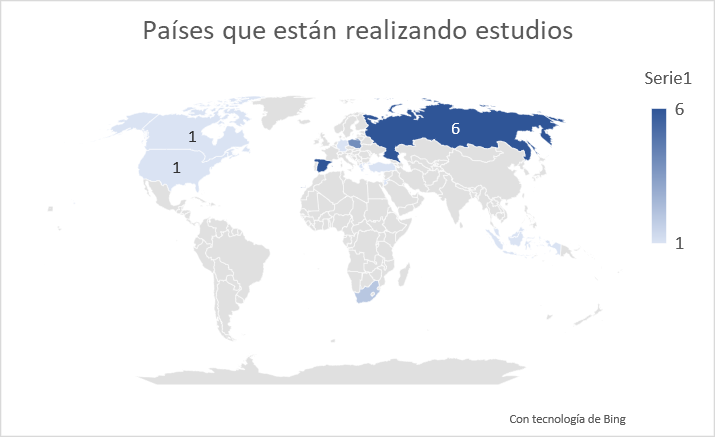
\includegraphics[width=\textwidth]{Fig6.png}
\caption{Países que están realizando estudios.}
\label{fig6}
\source{Elaboración propia.}
\end{minipage}
\end{figure}

\subsection{¿En qué contexto se desarrollan las investigaciones?}\label{sec-organizacao-latex}
La mayoría de las investigaciones analizadas se desarrollan en el contexto educativo, es decir, la muestra que participa en los estudios es en su mayoría estudiantes de primer ciclo, segundo ciclo y en un gran número estudiantes universitarios. Por otra parte, también son objeto de estudio las familias (tutores, padres, madres), niños y niñas (entre 9 y 11 años) adolescentes (personas entre 12 y 17 años) y adultos (de 18 años en adelante. Finalmente, cabe señalar que algunas de las investigaciones analizadas se basan en el análisis documental.

\begin{figure}[h!]
\centering
\begin{minipage}{0.65\textwidth}
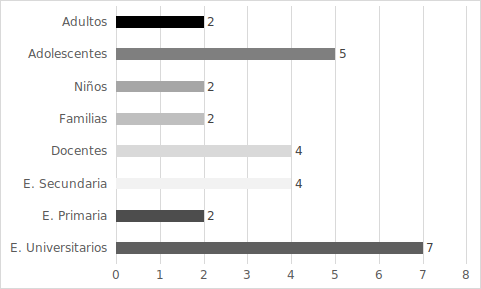
\includegraphics[width=\textwidth]{Fig7.png}
\caption{Muestra y contexto de investigación.}
\label{fig7}
\source{Elaboración propia.}
\end{minipage}
\end{figure}

En la \Cref{fig7} se observa que es en el ámbito universitario donde se centraliza la mayor parte de las investigaciones, seguidas de las centradas en adolescentes. También los docentes forman parte del interés investigador, así como las familias y estudiantes de educación secundaria.

\subsection{¿Cuáles son los principales resultados que han obtenido los estudios realizados?}\label{sec-titulo}
De los resultados obtenidos podemos destacar algunas ideas importantes:

\begin{enumerate}
    \item Dominar la cultura y ética digital ayuda a evitar conflictos por lo que es fundamental la formación y se pone el acento en la importancia de la formación de docentes y familias \cite{isrokatun2022digital}.
    \item Las familias y adultos ejercen una influencia importante a la hora de proveer entornos de aprendizaje seguros en línea y fuera de línea para los niños, así como creencias para aumentar su autoconciencia sobre la seguridad y el conocimiento de Internet. Estudios como \textcite{soldatova2020digital} concluyen que la brecha digital entre adolescentes y familias incide en las estrategias de mediación parental, se observa como las estrategias de control digital no son tan efectivas frente a las estrategias de mediación activa que proporciona una solución digital más fuerte y formas más constructivas de hacer frente a las amenazas del mundo digital y, riesgos en línea.
    \item Estudios centrados en adolescentes \cite{tomczyk_parents_2017} muestran que el conocimiento de padres y madres constituye un factor significativo a la hora de estar protegidos de las amenazas digitales, simultáneamente, debemos señalar que existe mayor necesidad de proporcionar formación a las familias para aumentar sus competencias digitales en el ámbito de la seguridad.
    \item Es necesaria la formación en ciudadanía digital en el ámbito universitario, pues los resultados revelan que los estudiantes universitarios no utilizan adecuadamente las tecnologías \cite{ogegbo2021assessment,takavarasha2018navigating}.
    \item Existe necesidad de formación en la competencia digital docente, asumiendo la escuela la responsabilidad formativa de parte de la población \cite{torres2022indicators}.
    \item Los estudios centrados en familia sugieren que estas todavía están inseguras sobre las aplicaciones informáticas y su selección \cite{mark2021invitation,schlebbe2018selecting}.
    \item Se sugiere que, para superar los factores de riesgo, es necesario desarrollar un sistema de entorno comunicativo y educativo seguro en los sistemas de educación secundaria y superior, siguiendo el impacto de la digitalización. Ello permitirá realizar un seguimiento eficaz de los factores riesgo y seleccionar las formas de aprendizaje más eficaces, teniendo en cuenta la individualización de las trayectorias educativas de los alumnos \cite{baeva2020safety,kaban2020secure}.
    \item Un análisis detallado de los resultados obtenidos por \textcite{potyrała2021teachers},  reveló que los docentes obtuvieron buenos resultados en la prueba en cuanto a su conocimiento sobre sexting y protección de imágenes, pero obtuvieron malas puntuaciones en cuanto a derechos de autor y la evaluación de la confiabilidad de la información en línea; los profesores varones saben más sobre los aspectos técnicos de la seguridad digital que las profesoras; los alumnos necesitan un apoyo especial en forma de educación informal y no formal.
    \item Hay estudios que revelan diferencias estadísticas en edad y género, siendo las chicas las que realizan más acciones de riesgo que no implican un deseo expreso de dañar a otras personas.
\end{enumerate}

\subsection{¿Qué perspectiva de futuro se presentan en los estudios analizados?}\label{sec-autores}
Se espera que la formación en seguridad digital se extienda en la educación superior, en especial a los futuros docentes, ya que son ellos los encargados de formar a las futuras generaciones, para la formación se destaca la importancia de las denominadas competencias blandas \cite{isrokatun2022digital,ogegbo2021assessment,takavarasha2018navigating}. De igual modo, los adultos (familias) deben asumir su responsabilidad para que los jóvenes realicen un uso seguro y ético por lo que la formación a familias se prevé como indispensable y necesaria. Hay que trazar puentes entre el entorno escolar y familiar \cite{mahadir_digital_2021}. En este sentido, \textcite{soldatova2020digital} propone la mediación activa de las familias, frente al control, como forma constructiva para hacer frente a las amenazas digitales. En algunos estudios se indica que la seguridad digital no se está tomando como indicador de la ciudadanía digital y es fundamental que en el futuro sea un elemento importante a tener en cuenta \cite{jwaifell2018proper}. Por otra parte, se propone que la formación en competencia digital sea integrada curricularmente de forma globalizada, atendiendo al área de seguridad digital de forma especial \cite{hazar2018digital}. Una vía para la formación comienza con la inclusión de esta competencia en los libros de texto \cite{kaban2020secure}. Otros autores ponen el acento en la capacidad formativa de la educación informal destacando de esta forma la eficacia de las estrategias colaborativas de aprendizaje informal \cite{quintana2020transmedia}. Finalmente, destacar que casi todas las investigaciones analizadas indican que es conveniente promover una mayor investigación sobre la llamada \textit{pedagogía de los medios} \cite{chelysheva2017basic}, ya que se considera que para minimizar los riesgos digitales hay que educar en ellos, se proponen futuras líneas de trabajo, encaminadas a dar respuesta a la demanda de una ciudadanía mejor preparada y más competente digitalmente \cite{arrufat2019competence,torres2019intervencion}.

\section{Discusión y conclusiones}\label{sec-idioma}
Teniendo en cuenta que el principal objetivo del estudio que se presenta ha sido explorar el estado de la cuestión sobre la seguridad digital tratada como parte de la competencia digital y la competencia digital docente, para detectar posibles lagunas que se están produciendo en la investigación de esta temática y así poder impulsar futuras líneas de investigación en las que hay que profundizar, queda patente que se reconoce la importancia de formar en la seguridad digital, pero el enfoque que se le está dando es muy genérico, ya que la mayoría se centra en protección en internet sin profundizar en aspectos concretos. En contrapartida, hay áreas de la competencia digital que no se tienen en cuenta como es el uso de internet y la protección medioambiental que, aunque hay algunas investigaciones realizadas al respecto, no se vinculan al ámbito de la competencia digital ciudadana y docente por lo que es necesario incidir en esta área para formar en el uso responsable y ecológico de las TIC.

Los resultados reflejan y confirman, la necesidad formativa para realizar usos seguros de internet y conocer los riesgos a los que nos expone. La responsabilidad formativa debe recaer en la familia y en las instituciones educativas por lo que es de vital importancia la formación de docentes y adultos. La educación debe abarcar todas las áreas que se reconcomen en los marcos competenciales, puesto que hasta el momento se ha contemplado de forma parcial. Los resultados reflejan también la necesidad de una mayor formación en el profesorado universitario ante la escasa Competencia Digital Docente, así como el desarrollo de las mismas en su propio alumnado. Es importante destacar, la necesidad de transferir las competencias en seguridad digital a entornos educativos no formales o informales, teniendo en cuenta que su uso, a veces se inicia antes en estos entornos que los formales.

En definitiva, podría afirmarse que no se está dando la importancia que debe a la formación en seguridad digital o se hace de forma parcial. El uso seguro de las tecnologías digitales se sigue dejando en manos de la autoformación de los jóvenes o del control de las familias que a veces no tienen competencias ni herramientas para asumir esa responsabilidad. La brecha digital generacional se interpone para la realización de una buena mediación tecnológica. Parece que está claro que el contexto educativo debe hacer frente a esta necesidad, pero de momento se encuentra vinculado a acciones aisladas y no a respuestas globales y reconocidas que encuentren reflejo en los marcos competenciales. Es esencial que las políticas educativas y los marcos de competencia aborden este desafío de manera más sistemática y efectiva para preparar a las generaciones futuras para enfrentar los desafíos del mundo digital con confianza y responsabilidad.

\section{Centros colaboradores}\label{sec-resumo}
El presente artículo es fruto de una estancia internacional y de una línea de investigación iniciada en colaboración entre la Escola Superior de Educação do Instituto Politécnico de Beja (Portugal) y la Universidad de Sevilla (España).



\printbibliography\label{sec-bib}
%conceptualization,datacuration,formalanalysis,funding,investigation,methodology,projadm,resources,software,supervision,validation,visualization,writing,review
\begin{contributors}[sec-contributors]
\authorcontribution{Raquel Barragán Sánchez}[conceptualization,datacuration,formalanalysis,investigation,methodology,validation,visualization,writing,review]
\authorcontribution{Luís Manuel da Cruz Murta}[methodology,supervision,visualization,writing,review]
\end{contributors}
\end{document}
